\chapter{Question 3}
\label{question-3}
\section{Question}

\begin{itemize}
\item Using 20 links that have TimeMaps
\begin{itemize}
\item With >= 20 mementos
\item Have existed \textgreater = 2 years (i.e., Memento-Datetime of “first memento” is April XX, 2013 or older)
\item Note: select from Q1/Q2 links, else choose them by hand
\end{itemize}
\item For each link, create a graph that shows Jaccard Distance, relative to the first memento, through time
	\begin{itemize}
		\item x-axis: continuous time, y-axis: Jaccard Distance relative to the first memento
	\end{itemize}
\end{itemize}


\section{Solution}
\begin{itemize}
\item I manually searched for the 20 URIs that satisfied the condition.
\item Then, I ran each of the URIs in the 20 TimeMaps through boilerpipe to retrieve the text. This would help me fetch the unigrams that I would then use to calculate the Jaccard Distance with respect to the first memento.
\item I modified the script from question one to calculate the Jaccard Distance.
\item Below are the graphs illustrating the Jaccard Distance relative to the first memento.
\end{itemize}

	\begin{minipage}{\linewidth}
		\centering
			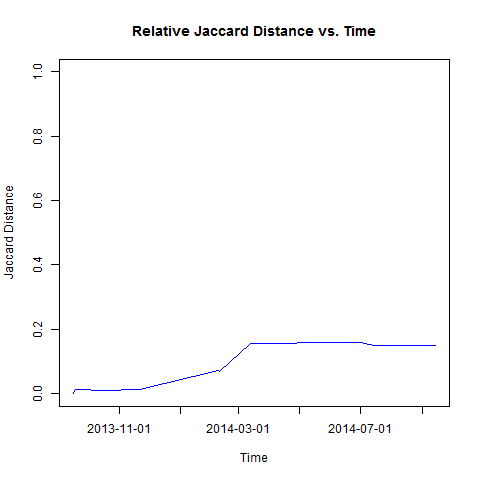
\includegraphics[scale=0.55]{figures/q3/uri1.png}
		\captionof{figure}{Jaccard Distance relative to first memento for URI\# 1}
		\label{wordCount}
	\end{minipage}

	\begin{minipage}{\linewidth}
		\centering
			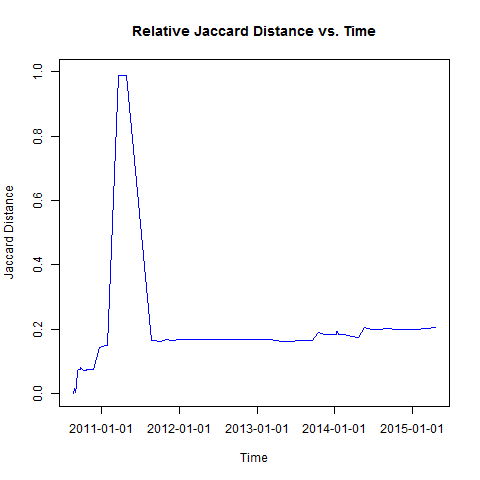
\includegraphics[scale=0.55]{figures/q3/uri2.png}
		\captionof{figure}{Jaccard Distance relative to first memento for URI\# 2}
		\label{wordCount}
	\end{minipage}
	
		\begin{minipage}{\linewidth}
		\centering
			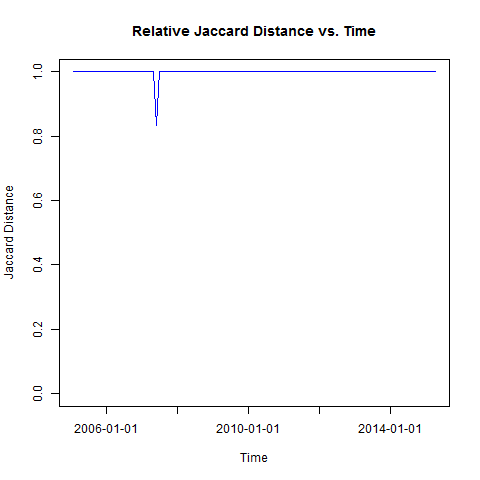
\includegraphics[scale=0.55]{figures/q3/uri3.png}
		\captionof{figure}{Jaccard Distance relative to first memento for URI\# 3}
		\label{wordCount}
	\end{minipage}
	
		\begin{minipage}{\linewidth}
		\centering
			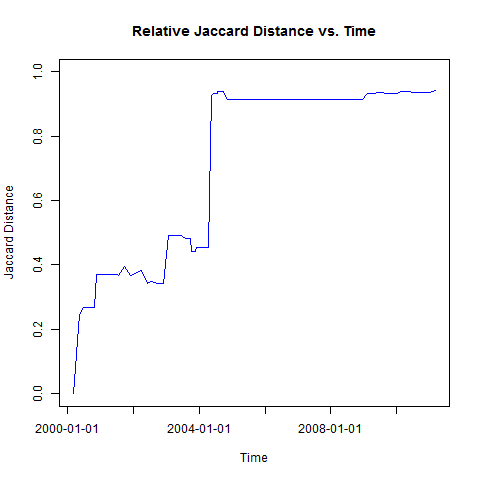
\includegraphics[scale=0.55]{figures/q3/uri4.png}
		\captionof{figure}{Jaccard Distance relative to first memento for URI\# 4}
		\label{wordCount}
	\end{minipage}
	
		\begin{minipage}{\linewidth}
		\centering
			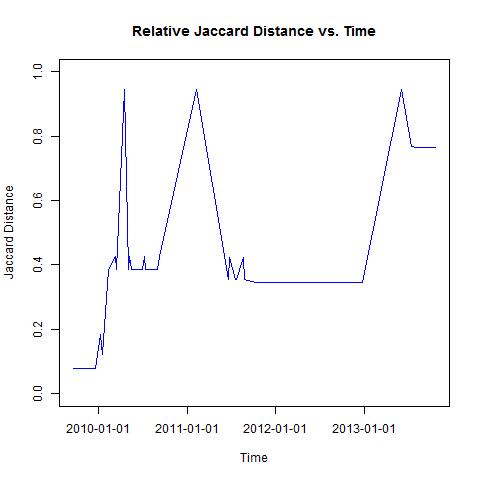
\includegraphics[scale=0.55]{figures/q3/uri5.png}
		\captionof{figure}{Jaccard Distance relative to first memento for URI\# 5}
		\label{wordCount}
	\end{minipage}
	
		\begin{minipage}{\linewidth}
		\centering
			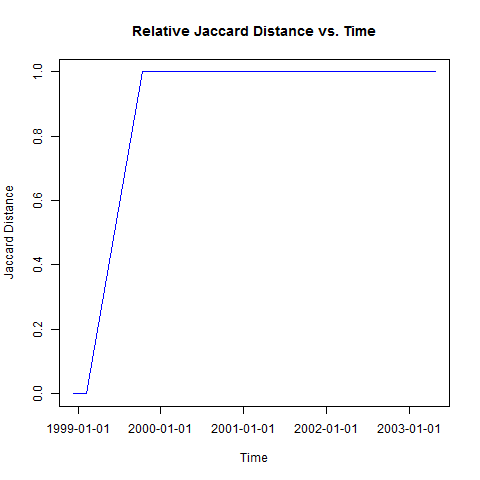
\includegraphics[scale=0.55]{figures/q3/uri6.png}
		\captionof{figure}{Jaccard Distance relative to first memento for URI\# 6}
		\label{wordCount}
	\end{minipage}
	
		\begin{minipage}{\linewidth}
		\centering
			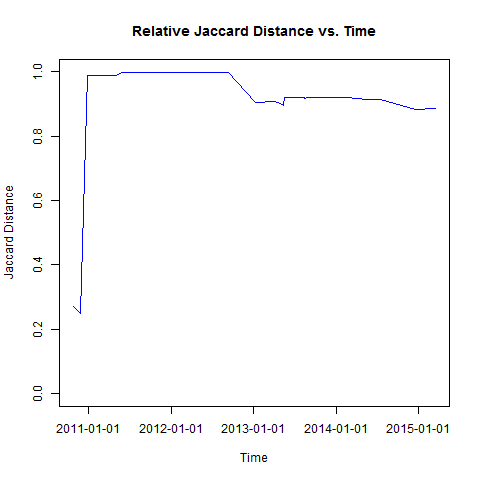
\includegraphics[scale=0.55]{figures/q3/uri7.png}
		\captionof{figure}{Jaccard Distance relative to first memento for URI\# 7}
		\label{wordCount}
	\end{minipage}
	
		\begin{minipage}{\linewidth}
		\centering
			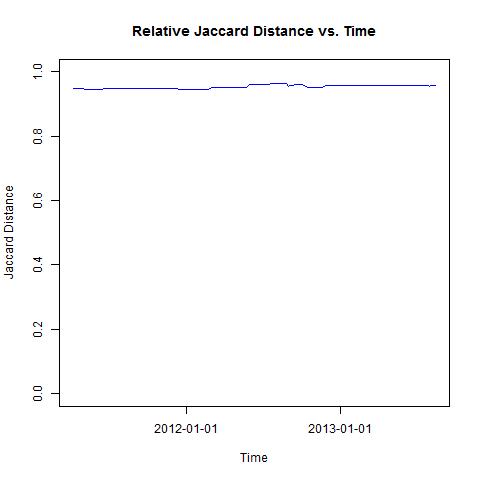
\includegraphics[scale=0.55]{figures/q3/uri8.png}
		\captionof{figure}{Jaccard Distance relative to first memento for URI\# 8}
		\label{wordCount}
	\end{minipage}
	
		\begin{minipage}{\linewidth}
		\centering
			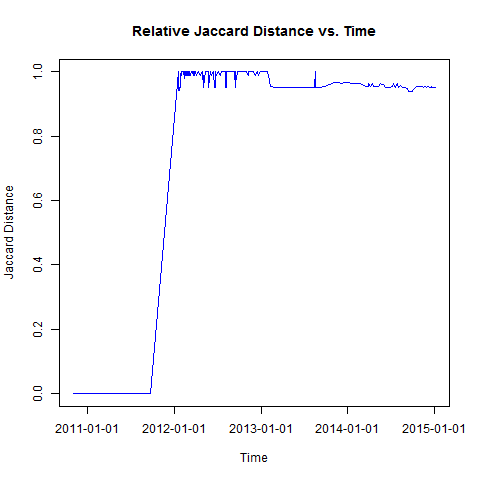
\includegraphics[scale=0.55]{figures/q3/uri9.png}
		\captionof{figure}{Jaccard Distance relative to first memento for URI\# 9}
		\label{wordCount}
	\end{minipage}
	
		\begin{minipage}{\linewidth}
		\centering
			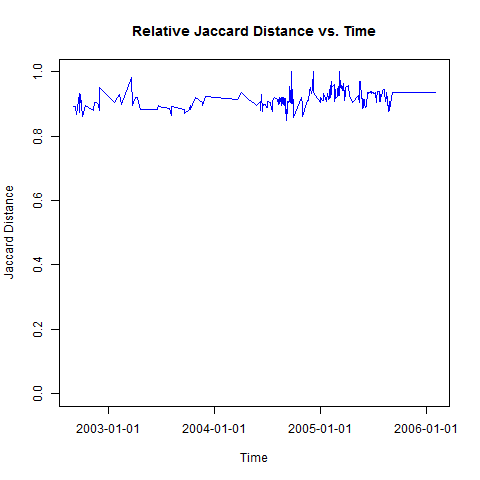
\includegraphics[scale=0.55]{figures/q3/uri10.png}
		\captionof{figure}{Jaccard Distance relative to first memento for URI\# 10}
		\label{wordCount}
	\end{minipage}
	
		\begin{minipage}{\linewidth}
		\centering
			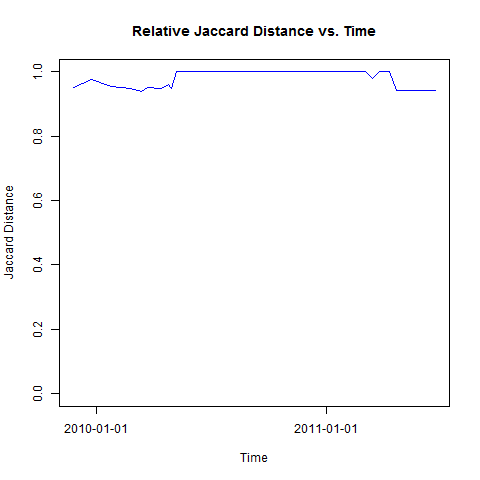
\includegraphics[scale=0.55]{figures/q3/uri11.png}
		\captionof{figure}{Jaccard Distance relative to first memento for URI\# 11}
		\label{wordCount}
	\end{minipage}
	
		\begin{minipage}{\linewidth}
		\centering
			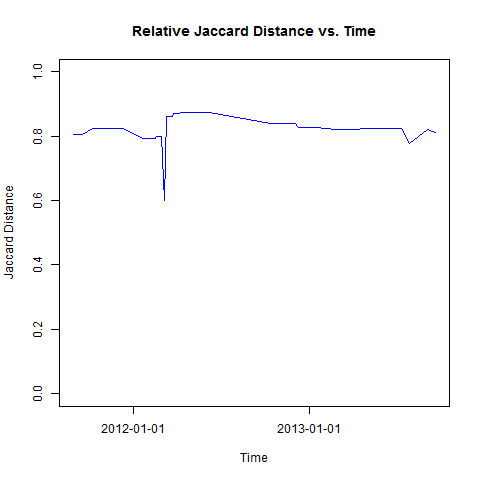
\includegraphics[scale=0.55]{figures/q3/uri12.png}
		\captionof{figure}{Jaccard Distance relative to first memento for URI\# 12}
		\label{wordCount}
	\end{minipage}
	
		\begin{minipage}{\linewidth}
		\centering
			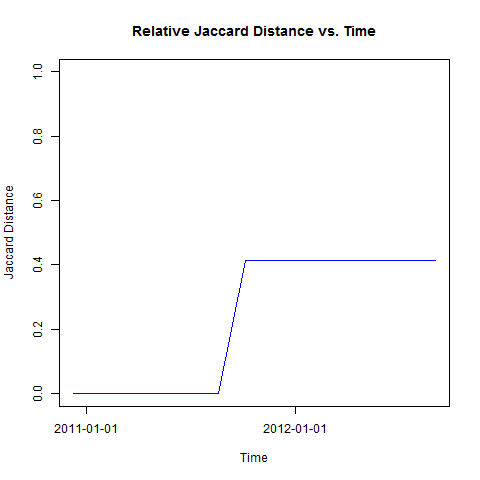
\includegraphics[scale=0.55]{figures/q3/uri13.png}
		\captionof{figure}{Jaccard Distance relative to first memento for URI\# 13}
		\label{wordCount}
	\end{minipage}
	
		\begin{minipage}{\linewidth}
		\centering
			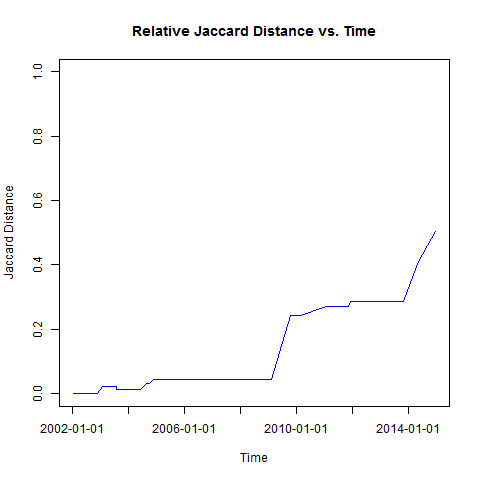
\includegraphics[scale=0.55]{figures/q3/uri14.png}
		\captionof{figure}{Jaccard Distance relative to first memento for URI\# 14}
		\label{wordCount}
	\end{minipage}
	
		\begin{minipage}{\linewidth}
		\centering
			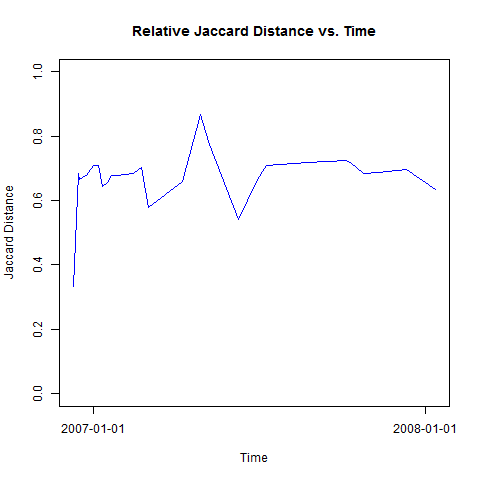
\includegraphics[scale=0.55]{figures/q3/uri15.png}
		\captionof{figure}{Jaccard Distance relative to first memento for URI\# 15}
		\label{wordCount}
	\end{minipage}
	
		\begin{minipage}{\linewidth}
		\centering
			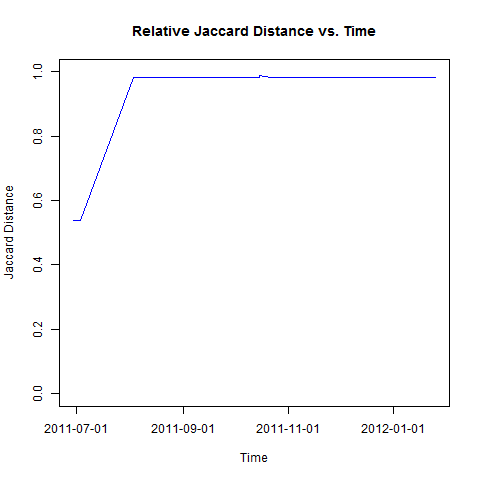
\includegraphics[scale=0.55]{figures/q3/uri16.png}
		\captionof{figure}{Jaccard Distance relative to first memento for URI\# 16}
		\label{wordCount}
	\end{minipage}
	
		\begin{minipage}{\linewidth}
		\centering
			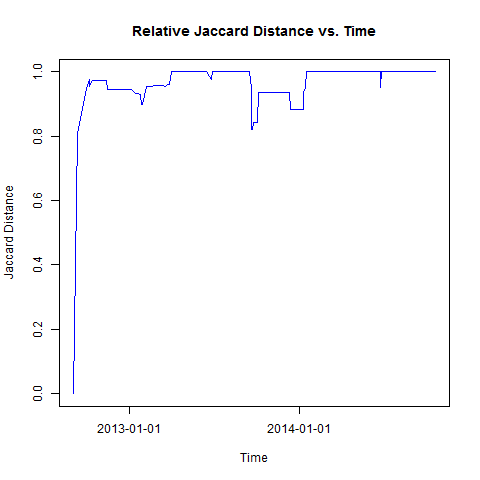
\includegraphics[scale=0.55]{figures/q3/uri17.png}
		\captionof{figure}{Jaccard Distance relative to first memento for URI\# 17}
		\label{wordCount}
	\end{minipage}
	
		\begin{minipage}{\linewidth}
		\centering
			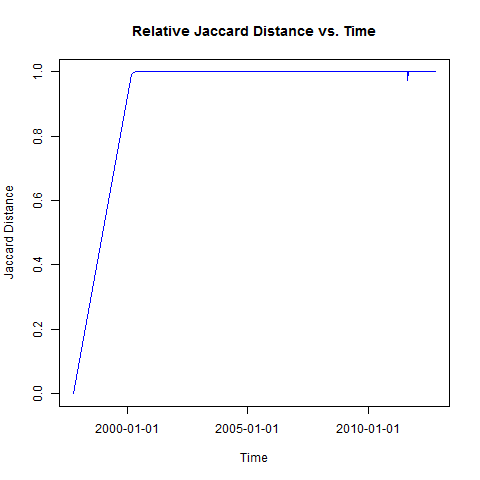
\includegraphics[scale=0.55]{figures/q3/uri18.png}
		\captionof{figure}{Jaccard Distance relative to first memento for URI\# 18}
		\label{wordCount}
	\end{minipage}
	
	\begin{minipage}{\linewidth}
		\centering
			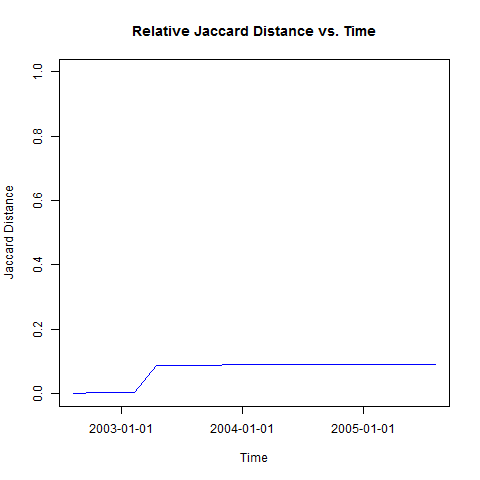
\includegraphics[scale=0.55]{figures/q3/uri19.png}
		\captionof{figure}{Jaccard Distance relative to first memento for URI\# 19}
		\label{wordCount}
	\end{minipage}
	
	\begin{minipage}{\linewidth}
		\centering
			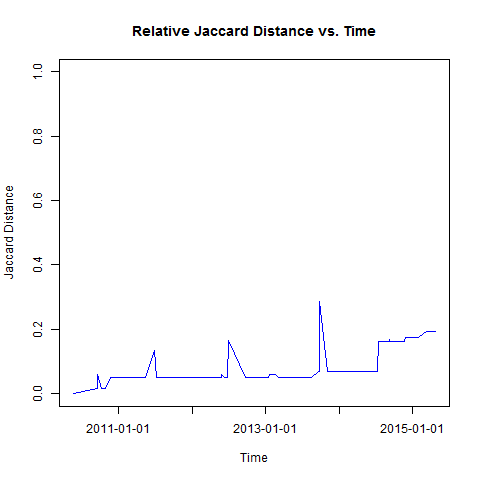
\includegraphics[scale=0.55]{figures/q3/uri20.png}
		\captionof{figure}{Jaccard Distance relative to first memento for URI\# 20}
		\label{wordCount}
	\end{minipage}

\newpage
\section{Code Listing}

\lstinputlisting[language=Python,breaklines = true,frame=single,caption={Python program for fetching boilerpipe content for each memento in the TimeMap.},label=lst:q1-1,captionpos=b,numbers=left,showspaces=false,showstringspaces=false,basicstyle=\footnotesize]{pythonFiles/getMementoBoilerPlate.py}

\newpage
\lstinputlisting[language=Python,breaklines = true,frame=single,caption={Python program for calculating the Jaccard Distance relative to first memento.},label=lst:q1-1,captionpos=b,numbers=left,showspaces=false,showstringspaces=false,basicstyle=\footnotesize]{pythonFiles/getMementoNGrams.py}

\newpage
\lstinputlisting[language=R,breaklines = true,frame=single,caption={R program for generating plot for Jaccard Distance vs. Time}, label=lst:q1R1,captionpos=b,numbers=left,showspaces=false,showstringspaces=false,basicstyle=\footnotesize]{rFiles/q3.R}